%%%%%%%%%%%%%%%%%%%%%%%%%%%%%%%%%%%%%%%%%
% McMaster Masters/Doctoral Thesis
% LaTeX Template
% Version 2.2 (11/23/15)
%
% This template has been downloaded from:
% http://www.LaTeXTemplates.com
% Then subsequently from http://www.overleaf.com
%
% Version 2.0 major modifications by:
% Vel (vel@latextemplates.com)
%
% Original authors:
% Steven Gunn  (http://users.ecs.soton.ac.uk/srg/softwaretools/document/templates/)
% Sunil Patel (http://www.sunilpatel.co.uk/thesis-template/)
%
% Modified to McMaster format by Benjamin Furman (contact: https://www.xenben/com; Most up
% to date template at https://github.com/benjaminfurman/McMaster_Thesis_Template,
% occasionally updated on Overleaf template page)
%
% Modified for macdown by Antonio Paez; most up to date version at https://github.com/paezha/macdown
%
% License:
% CC BY-NC-SA 3.0 (http://creativecommons.org/licenses/by-nc-sa/3.0/)
%
%%%%%%%%%%%%%%%%%%%%%%%%%%%%%%%%%%%%%%%%%

%----------------------------------------------------------------------------------------
% DOCUMENT CONFIGURATIONS
%----------------------------------------------------------------------------------------

\documentclass[
11pt, % The default document font size, options: 10pt, 11pt, 12pt
oneside, % Two side (alternating margins) for binding by default, uncomment to switch to one side
english, % other languages available
singlespacing, % Single line spacing, alternatives: onehalfspacing or doublespacing
%draft, % Uncomment to enable draft mode (no pictures, no links, overfull hboxes indicated)
%nolistspacing, % If the document is onehalfspacing or doublespacing, uncomment this to set spacing in lists to single
%liststotoc, % Uncomment to add the list of figures/tables/etc to the table of contents
%toctotoc, % Uncomment to add the main table of contents to the table of contents
]{macthesis} % The class file specifying the document structure

%----------------------------------------------------------------------------------------
% Import packages here
%----------------------------------------------------------------------------------------
\usepackage[utf8]{inputenc} % Required for inputting international characters
\usepackage[T1]{fontenc} % Output font encoding for international characters
\usepackage{lastpage} % count pages
\usepackage{lmodern} % could change font type by calling a different package
\usepackage{lscape} % for landscaping pages
% New commands for landscape orientation
\newcommand{\blandscape}{\begin{landscape}}
\newcommand{\elandscape}{\end{landscape}}
%
\usepackage{siunitx} % for scientific units (micro-liter, etc)
\setcounter{tocdepth}{2} % so that only section and sub sections appear in Table of Contents. Remove or set depth to 3 to include sub-sub-sections

%----------------------------------------------------------------------------------------
% Define a blank page
%----------------------------------------------------------------------------------------
\def\blankpage{%
      \clearpage%
      \thispagestyle{empty}%
      \addtocounter{page}{-1}%
      \null%
      \clearpage}

%----------------------------------------------------------------------------------------
% Define a tight list
%----------------------------------------------------------------------------------------
\def\tightlist{}

%----------------------------------------------------------------------------------------
%	Highlight Code Chunks
%----------------------------------------------------------------------------------------
  \usepackage{color}
  \usepackage{fancyvrb}
  \newcommand{\VerbBar}{|}
  \newcommand{\VERB}{\Verb[commandchars=\\\{\}]}
  \DefineVerbatimEnvironment{Highlighting}{Verbatim}{commandchars=\\\{\}}
  % Add ',fontsize=\small' for more characters per line
  \usepackage{framed}
  \definecolor{shadecolor}{RGB}{248,248,248}
  \newenvironment{Shaded}{\begin{snugshade}}{\end{snugshade}}
  \newcommand{\AlertTok}[1]{\textcolor[rgb]{0.94,0.16,0.16}{#1}}
  \newcommand{\AnnotationTok}[1]{\textcolor[rgb]{0.56,0.35,0.01}{\textbf{\textit{#1}}}}
  \newcommand{\AttributeTok}[1]{\textcolor[rgb]{0.13,0.29,0.53}{#1}}
  \newcommand{\BaseNTok}[1]{\textcolor[rgb]{0.00,0.00,0.81}{#1}}
  \newcommand{\BuiltInTok}[1]{#1}
  \newcommand{\CharTok}[1]{\textcolor[rgb]{0.31,0.60,0.02}{#1}}
  \newcommand{\CommentTok}[1]{\textcolor[rgb]{0.56,0.35,0.01}{\textit{#1}}}
  \newcommand{\CommentVarTok}[1]{\textcolor[rgb]{0.56,0.35,0.01}{\textbf{\textit{#1}}}}
  \newcommand{\ConstantTok}[1]{\textcolor[rgb]{0.56,0.35,0.01}{#1}}
  \newcommand{\ControlFlowTok}[1]{\textcolor[rgb]{0.13,0.29,0.53}{\textbf{#1}}}
  \newcommand{\DataTypeTok}[1]{\textcolor[rgb]{0.13,0.29,0.53}{#1}}
  \newcommand{\DecValTok}[1]{\textcolor[rgb]{0.00,0.00,0.81}{#1}}
  \newcommand{\DocumentationTok}[1]{\textcolor[rgb]{0.56,0.35,0.01}{\textbf{\textit{#1}}}}
  \newcommand{\ErrorTok}[1]{\textcolor[rgb]{0.64,0.00,0.00}{\textbf{#1}}}
  \newcommand{\ExtensionTok}[1]{#1}
  \newcommand{\FloatTok}[1]{\textcolor[rgb]{0.00,0.00,0.81}{#1}}
  \newcommand{\FunctionTok}[1]{\textcolor[rgb]{0.13,0.29,0.53}{\textbf{#1}}}
  \newcommand{\ImportTok}[1]{#1}
  \newcommand{\InformationTok}[1]{\textcolor[rgb]{0.56,0.35,0.01}{\textbf{\textit{#1}}}}
  \newcommand{\KeywordTok}[1]{\textcolor[rgb]{0.13,0.29,0.53}{\textbf{#1}}}
  \newcommand{\NormalTok}[1]{#1}
  \newcommand{\OperatorTok}[1]{\textcolor[rgb]{0.81,0.36,0.00}{\textbf{#1}}}
  \newcommand{\OtherTok}[1]{\textcolor[rgb]{0.56,0.35,0.01}{#1}}
  \newcommand{\PreprocessorTok}[1]{\textcolor[rgb]{0.56,0.35,0.01}{\textit{#1}}}
  \newcommand{\RegionMarkerTok}[1]{#1}
  \newcommand{\SpecialCharTok}[1]{\textcolor[rgb]{0.81,0.36,0.00}{\textbf{#1}}}
  \newcommand{\SpecialStringTok}[1]{\textcolor[rgb]{0.31,0.60,0.02}{#1}}
  \newcommand{\StringTok}[1]{\textcolor[rgb]{0.31,0.60,0.02}{#1}}
  \newcommand{\VariableTok}[1]{\textcolor[rgb]{0.00,0.00,0.00}{#1}}
  \newcommand{\VerbatimStringTok}[1]{\textcolor[rgb]{0.31,0.60,0.02}{#1}}
  \newcommand{\WarningTok}[1]{\textcolor[rgb]{0.56,0.35,0.01}{\textbf{\textit{#1}}}}

%----------------------------------------------------------------------------------------
% Handling Citations
%----------------------------------------------------------------------------------------

% definitions for citeproc citations
\NewDocumentCommand\citeproctext{}{}
\NewDocumentCommand\citeproc{mm}{%
\begingroup\def\citeproctext{#2}\cite{#1}\endgroup}
\makeatletter
% allow citations to break across lines
\let\@cite@ofmt\@firstofone
% avoid brackets around text for \cite:
\def\@biblabel#1{}
\def\@cite#1#2{{#1\if@tempswa , #2\fi}}
\makeatother
\newlength{\cslhangindent}
\setlength{\cslhangindent}{1.5em}
\newlength{\csllabelwidth}
\setlength{\csllabelwidth}{3em}
\newenvironment{CSLReferences}[2] % #1 hanging-indent, #2 entry-spacing
{\begin{list}{}{%
	\setlength{\itemindent}{0pt}
	\setlength{\leftmargin}{0pt}
	\setlength{\parsep}{0pt}
	% turn on hanging indent if param 1 is 1
	\ifodd #1
	\setlength{\leftmargin}{\cslhangindent}
	\setlength{\itemindent}{-1\cslhangindent}
	\fi
	% set entry spacing
	\setlength{\itemsep}{#2\baselineskip}}}
{\end{list}}
\usepackage{calc}
\newcommand{\CSLBlock}[1]{\hfill\break\parbox[t]{\linewidth}{\strut\ignorespaces#1\strut}}
\newcommand{\CSLLeftMargin}[1]{\parbox[t]{\csllabelwidth}{\strut#1\strut}}
\newcommand{\CSLRightInline}[1]{\parbox[t]{\linewidth - \csllabelwidth}{\strut#1\strut}}
\newcommand{\CSLIndent}[1]{\hspace{\cslhangindent}#1}


%----------------------------------------------------------------------------------------
% Collect all your header information from the chapters here, things like acronyms, custom commands, necessary packages, etc.
%----------------------------------------------------------------------------------------
\usepackage{parskip} %this will put spaces between paragraphs
\setlength{\parindent}{15pt} % this will create and indent on all but the first paragraph of each section.
% should maybe change to glossaries package
\usepackage{acro}
\DeclareAcronym{est}{
	short = EST,
	long  = expressed sequence tags
}

\DeclareAcronym{Xl}{
	short = \textit{X.~laevis},
	long  = \textit{Xenopus~laevis}
}
\DeclareAcronym{Xg}{
	short = \textit{X.~gilli},
	long  = \textit{Xenopus~gilli}
}

\usepackage{etoolbox}
\preto\chapter{\acresetall} % resets acronyms for each chapter

\usepackage{xspace} %helps spacing with custom commands.
\newcommand{\oddname}{{\sc SoME goOfY LonG ThiNg With an AwkWarD NAme}\xspace}


\usepackage{pgfplotstable} % a much better way to handle tables
\pgfplotsset{compat=1.12}

% \usepackage{float} % if you need to demand figure/table placement, then this will allow you to use [H], which demands a figure placement. Beware, making LaTeX do things it doesn't want may lead to oddities.


%%%%
% LINK COLORS
% You can control the link colors at the end of the McMasterThesis.cls file. There is also a true/false option there to turn off all link colors.
%%%%


%----------------------------------------------------------------------------------------
%	THESIS INFORMATION
%----------------------------------------------------------------------------------------

\title{GEOG712 Course Project - Assessing the influence of tourists' perceived travel environment and their travel behavior on travel satisfaction using structural equation models (SEM): a case of Qinghai-Tibet Plateau}
%\thesistitle{Thesis Title} % Your thesis title, print it elsewhere with \ttitle
\author{Haoran Xu}
%\author{John \textsc{Smith}} % Your name, print it elsewhere with \authorname
\bdegree{B.Sc.}
\mdegree{}
%Previous degrees % print it elsewhere with \bdeg and \mdeg
\date{}
% The month and year that you submit your FINAL draft TO THE LIBRARY (May or December)
\university{McMaster University}
%\university{\href{http://www.mcmaster.ca/}{McMaster University}} % Your university's name and URL, print it elsewhere with \univname
%\division{}
\faculty{Faculty of Science} % Your faculty's name and URL, print it elsewhere with \facname
\department{School of Earth, Environment and Society} % Your department's name and URL, print it elsewhere with \deptname
\subject{Geography} % Your subject area, print it elsewhere with \subjectname
%\group{\href{http://researchgroup.university.com}{Research Group Name}} % Your research group's name and URL, print it elsewhere with \groupname
\supervisor{}
%\supervisor{Dr. Jane \textsc{Smith}} % Your supervisor's name, print it elsewhere with \supname
\examiner{} % Your examiner's name, print it elsewhere with \examname
\degree{Doctor of Philosophy}
%\degree{Doctor of Philosophy} % Your degree name, print it elsewhere with \degreename
\addresses{} % Your address, print it elsewhere with \addressname
\keywords{} % Keywords for your thesis, print it elsewhere with \keywordnames


% this sets up hyperlinks
\hypersetup{pdftitle=\ttitle} % Set the PDF's title to your title
\hypersetup{pdfauthor=\authorname} % Set the PDF's author to your name
\hypersetup{pdfkeywords=\keywordnames} % Set the PDF's keywords to your keywords

\begin{document}
\sloppy

\frontmatter % Use roman page numbering style (i, ii, iii, iv...) for the pre-content pages

\pagestyle{plain} % Default to the plain heading style until the thesis style is called for the body content

%----------------------------------------------------------------------------------------
%	Half Title (lay title)
%----------------------------------------------------------------------------------------
%\begin{halftitle} % could not get this environment working
%\vspace*{\fill}
\vspace{6cm}
\begin{center}
\ttitle
\end{center}
%\vspace*{\fill}
\pagenumbering{gobble} % leave this here, McMaster doesn't want this page numbered
%\end{halftitle}
\clearpage

%----------------------------------------------------------------------------------------
%	TITLE PAGE
%----------------------------------------------------------------------------------------
\pagenumbering{gobble}
\begin{center}

\vfill
\textsc{\Large \ttitle} \\

\vfill
{By \authorname\, \bdeg }


 \vfill
{\large \textit{A Thesis Submitted to the School of Graduate Studies in the Partial Fulfillment of the Requirements for the Degree \degreename}}\\

\vfill
{\large \univname\, \copyright\, Copyright by \authorname\, \today}\\[4cm] % replace \today with the submission date

\end{center}
\blankpage
\clearpage

%----------------------------------------------------------------------------------------
%	QUOTATION PAGE
%----------------------------------------------------------------------------------------

\vspace*{0.2\textheight}

\noindent{\itshape Hope in 2025 you can code more, better, and with confidence.}\bigbreak

\hfill\textemdash Haoran

\blankpage
\clearpage

%%%%%%%%%%%%%%%%%%%%%%%%%%%
%%%%%%%%%%%%%%%%%%%%%%%%%%%
% optional page stuff
%----------------------------------------------------------------------------------------
% can do physical constraints and symbols pages, see the original thesis example on overleaf if you want to include them at https://www.overleaf.com/latex/templates/template-for-a-masters-slash-doctoral-thesis/mkzrzktcbzfl#.VlPeicorpE4
%----------------------------------------------------------------------------------------

%----------------------------------------------------------------------------------------
%	DEDICATION
%----------------------------------------------------------------------------------------


\blankpage
\clearpage


%----------------------------------------------------------------------------------------
%	Descriptive note numbered ii
%----------------------------------------------------------------------------------------
% Need to add below info
\newpage
\pagenumbering{roman} % leave to turn numbering back on
\setcounter{page}{2} % leave here to make this page numbered ii, a Grad School requirement

\noindent % stops indent on next line
\univname \\
\degreename\, (\the\year) \\
Hamilton, Ontario (\deptname) \\[1.5cm]
TITLE: \ttitle \\
AUTHOR: \authorname\,  %list previous degrees
(\univname)  \\
SUPERVISOR: \supname\, \\
NUMBER OF PAGES: \pageref{lastoffront}, \pageref{LastPage}  % put in iv and number

\clearpage

%----------------------------------------------------------------------------------------
%	Lay abstract number iii
%----------------------------------------------------------------------------------------
% not actually included in most theses, though requested by the GSA
% uncomment below lines if you want to include one
\section*{Lay Abstract}
  This r project \texttt{TravelBehaviorQinghai} is created by first-year PhD student Haoran Xu to produce a model paper for the final course project of ``GEOG712 - Reproducible Research Workflow'', taught by Dr.~Antonio Paez at McMaster University, Canada.
\blankpage
\clearpage


%----------------------------------------------------------------------------------------
%	ABSTRACT PAGE number iv
%----------------------------------------------------------------------------------------

\section*{\Huge Abstract}
\addchaptertocentry{\abstractname}
% Type your abstract here.
The study probes into how factors as travel behavior and perceived travel environment can influence tourists' travel satisfaction on Qinghai-Tibet Pleateau. The single-group SEM analysis conducted in this model peper revealed mixed effects across different pathways. Perceived tourist attraction environment significantly influenced travel satisfaction, while perceived road environment had no notable direct effect. Mediating effects showed that better tourist site conditions led to longer daily travel distances, whereas worse road conditions reduced travel distance. Travel modes exhibited minimal direct effects on satisfaction, with walking positively contributing and car driving by others showing the largest negative impact. Regarding travel behavior, frequency of travel to the Qinghai-Tibet Plateau had a minor positive effect on satisfaction, although insignificant, and daily travel distance showed no direct association.
\blankpage
\clearpage

%----------------------------------------------------------------------------------------
%	ACKNOWLEDGEMENTS
%----------------------------------------------------------------------------------------

  \begin{acknowledgements}
  \addchaptertocentry{\acknowledgementname} % Add the acknowledgments to the table of contents
    I would like to thank Dr.~Huaxiong Jiang and my undergrad fellows in old days for helping me with research design and questionnaire distributing. I would also like to thank Dr.~Antonio Paez for teaching this course and guiding me throughout the whole semester to learn from scratch about R and Github. With limited coding experiences before, I had been exposed to a lot of new ideas and thoughts on doing research itself. Mostly importantly, I am glad that I got to have the chance to build my own coding space little by little through detailed instructions, and that I could have little more confidence in coding skills instead of anxiety and upset. Anyways, this course surely would shed a very important light in my subsequent years of pursuing a PhD and a possible academic career.
  \end{acknowledgements}
\blankpage
\clearpage

%----------------------------------------------------------------------------------------
%	LIST OF CONTENTS/FIGURES/TABLES PAGES
%----------------------------------------------------------------------------------------

\tableofcontents % Prints the main table of contents

\listoffigures % Prints the list of figures

\listoftables % Prints the list of tables

%----------------------------------------------------------------------------------------
%	ABBREVIATIONS
%----------------------------------------------------------------------------------------
% many theses don't use this section, as it will be declared at first use and again each chapter. Uncomment these four lines to activate if you want
%\clearpage
%\section*{\Huge Acronyms}
%\addchaptertocentry{Acronyms}
%\printacronyms[name] % name without an option stops the header

%----------------------------------------------------------------------------------------
%	DECLARATION PAGE
%----------------------------------------------------------------------------------------

\begin{declaration}
\addchaptertocentry{\authorshipname}

\noindent I, \authorname, declare that this thesis titled, \emph{\ttitle} and the work presented in it are my own. I confirm that:

I did most of the research.

Also the writting.

Sometimes I cried.

But mostly I had fun.

\end{declaration}


%----------------------------------------------------------------------------------------
% The following bit is just here to make sure we end up on a new page and get the total number of roman numeral
\label{lastoffront}
\clearpage
% make sure this command is on the last of your frontmatter pages, i.e. only this command, a \clearpage then \mainmatter
% should be fine without modification
%----------------------------------------------------------------------------------------

%----------------------------------------------------------------------------------------
%	THESIS MAIN BODY
%----------------------------------------------------------------------------------------

\mainmatter % here the regular arabic numbering starts
\pagestyle{thesis}
\chapter*{Preface}\label{preface}
\addcontentsline{toc}{chapter}{Preface}

This r project \texttt{TravelBehaviorQinghai} is created by first-year PhD student \href{https://github.com/Horan517}{Haoran Xu} to produce a model paper for the final course project of \href{https://github.com/paezha/Reproducible-Research-Workflow/tree/master}{``GEOG712 - Reproducible Research Workflow''}, taught by \href{https://experts.mcmaster.ca/display/paezha}{Dr.~Antonio Paez} at McMaster University, Canada.

The paper is titled ``Assessing the influence of tourists' perceived travel environment and their travel behavior on travel satisfaction using structural equation models (SEM): a case of Qinghai-Tibet Plateau'', and stems from a half-way done research project in collaboration with \href{https://www.researchgate.net/scientific-contributions/Huaxiong-Jiang-2157090528}{Dr.~Huaxiong Jiang} starting from Jun, 2022 from \href{https://english.bnu.edu.cn/}{Beijing Normal Universtiy, China}.

The project paused since March of 2023 due to lack of time and energy investment. Therefore, I am taking the chance of this course project to review and re-arrange the previous work I had done nearly two years ago. Main work I did for this course project include:

\begin{itemize}
\tightlist
\item
  developing an r package called \href{https://github.com/Horan517/TravelBehaviorQinghaiData}{``TravelBehaviorQinghaiData''} using existing data in Excel format, transforming it into reproducible, open-sourced, and well-cleaned .rda format data.
\item
  using r package \href{https://lavaan.ugent.be/}{lavaan} to reproduce the \href{https://en.wikipedia.org/wiki/Structural_equation_modeling}{Structural Equations Modeling} (SEM) method, which was previously constructed and performed in a commercial software called \href{https://www.statmodel.com/}{mplus}.
\item
  first time writing a model article in r studio using latex syntax, in which I practiced several r packages such as \texttt{tidyverse}, \texttt{kableExtra}, and \texttt{macdown}, \href{https://github.com/paezha/macdown?tab=readme-ov-file}{a template for writing a McMaster graduate thesis}.
\end{itemize}

Citing format: Xu, H. (2024). TBQTSEM: a model paper of ``Assessing the influence of tourists' perceived travel environment and their travel behavior on travel satisfaction using structural equation models (SEM): a case of Qinghai-Tibet Plateau''. \url{https://github.com/Horan517/TBQTSEM}

\chapter{Introduction}\label{rmd-basics}

\section{Introduction}\label{introduction}

Subjective well-being is the psychological assessment of people's lives, including their emotional response to incidents and cognitive perceptions on life quality (Diener, 2000). The shift of well-being assessment from merely evaluating objective elements (wealth etc.) to incorporating multiple subjective indicators of assessment occurs in recent times as previous methods fail to determine the quality of life (De Vos, 2019; McCabe \& Johnson, 2013).

The relationships of tourism and SWB has been an emerging interest for many scholars to dig into. There are firm evidence that indicates tourism generally contributes to social tourists' well-being (McCabe \& Johnson, 2013). Scholars often use two-step surveys to explore the effect outdoor travel has on well-being improvement. Whilst another line of research focuses on the intrinsic mechanisms of the relationship, probing into how possible factors of tourism like built environment and travel behavior affect trip satisfaction and its internal interaction effects (Carneiro \& Eusébio, 2019). While among the varied indicators of detecting respondents' SWB, satisfaction is an effective factor to represent people's perceived subjective feeling towards a either short or long activity (Chen, Fan, Cao, \& Khattak, 2019).

This study digs into the relationships between travel satisfaction and other factors such as travel modes, travel frequency, travel distance and tourists' perceived tourist attraction environment and road environment. The core research questions is: what kind of factors would greatly impact local and non-local tourists' travel behavior and their travel satisfaction on Qinghai-Tibet Plateau.

\chapter{Data \& Methodology}\label{rmd-basics}

\section{Study Area and Data Collection}\label{study-area-and-data-collection}

The study area, Qinghai-Tibet Plateau, or referred to as Tibetan Plateau, is situated in the western region of China and characterized by its high altitude averaging over 4,000 meters. Due to its low population density and an extremely alpine climate, it exhibits a unique set of travel behavioral patterns for local residents or outside tourists. Furthermore, in recent years, the plateau has witnessed rapid infrastructural development invested by Chinese government, and a significant surge in tourist influx (Gao \& Sun, 2021). Despite this growth, scholarly investigations into travel behaviors, satisfaction levels, and the broader implications of these developments on local and visiting populations remain scant.

The questionnaire-collecting process started both online and on-site in July of 2022. The online questionnaires were written on the cover page that only those who had ever been to Qinghai-Tibet Plateau were qualified to fill out them. Then followed by was the on-site questionnaire-distributing process along with the Second Tibetan Plateau Scientific Expedition and Research Program during late July to early August. To specifically target at tourists while considering the convenience of conducting investigation, we mainly chose four touristic sites to collect questionnaires along the expedition route. Eventually, we collected 729 on-site questionnaires, which were acquired mostly in four sites - Qinghai Province Museum in Xining City, Qinghai Lake Scenic Area, Dachaidan Emerald Lake Scenic Area, Mani Stone Mound Scenic Area in Yushu City (Figure \ref{fig:SampleLocations}). With a total number of 830 questionnaires, 16 were filtered out due to a lot of missing answers, leaving 814 eventually entering modeling phase, with an validity rate of 98.07\%.

\begin{figure}

{\centering 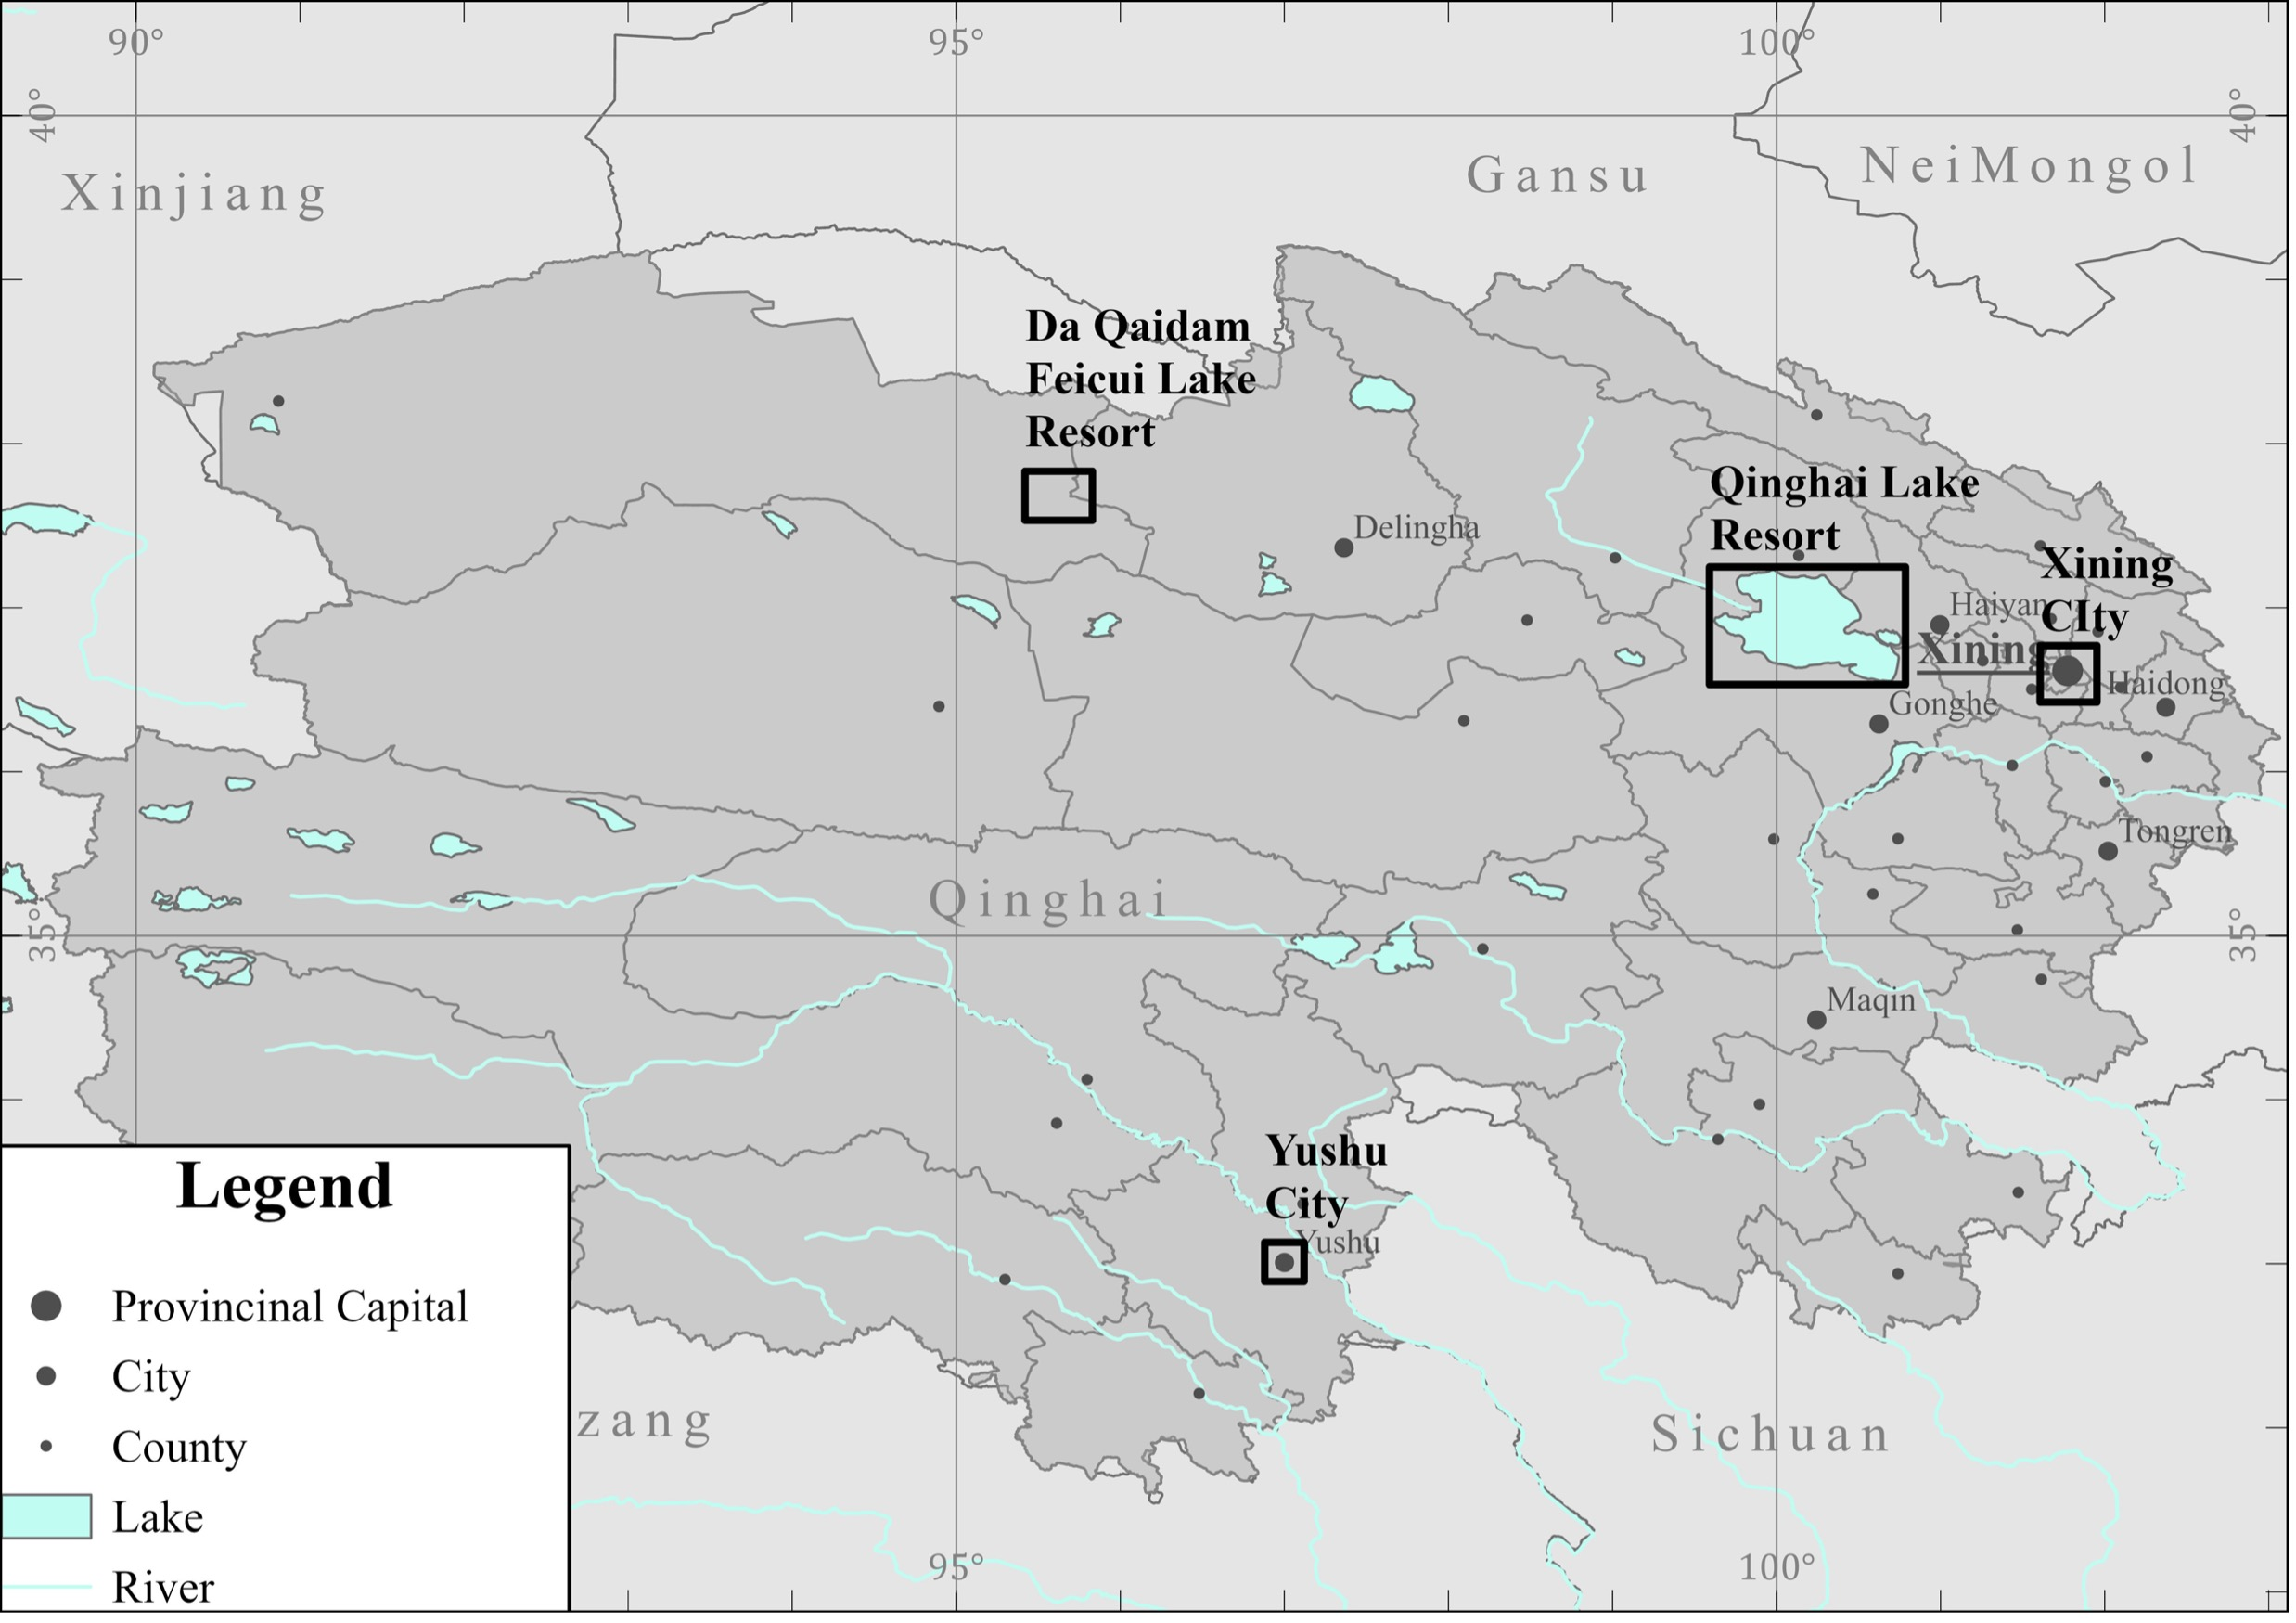
\includegraphics[width=0.8\linewidth]{figure/SampleLocations} 

}

\caption{\label{fig:SampleLocations}Sampling Locations on the Qinghai-Tibet Plateau}\label{fig:fig1-sample-locations}
\end{figure}

\section{Variables}\label{variables}

The survey was originally designed in the contexts of assessing smart transportation within the Qinghai-Tibet Plateau, which contains multifaceted aspects spanning from travel behavior, travel perceptions to technology adoption and usage. This study focuses only on several key dimensions, which are tourist travel behavior, their perceived travel environment, travel satisfaction, and their socio-demograpical characteristics.

The complete questionnaire (originally in Chinese and translated in English) alongside with data cleaning and re-digitalizing is stored in \texttt{TravelBehaviorQinghaiData} \href{https://github.com/Horan517/TravelBehaviorQinghaiData}{package}.

Specifically, socio-demograpical variables include gender, age, residence, personal monthly income, education level, profession, household size and ownership of driving license. Travel behavior variables in this model include frequency of traveling to Qinghai-Tibet Plateau in the past year and average daily traveling distance during the trip people were having when filling the questionnaire. Travel expectation and travel satisfaction are also measured, using a 5-point Likert scale ranging from strongly agree (value = 5) to strongly disagree (value = 1). Lastly, travel environment variables include two latent variables - people's perceptions of the environment of tourist attractions and the environment of roads along the trip, with the first consisting of 6 questions and the latter consisting of 5 questions.

\section{Methodology}\label{methodology}

Structural Equation Model (SEM) was used in the study to entangle the complex relationships across different variables. According to Bollen (1989), SEM is able to simultaneously estimate the causal relationships among a set of observed variables based on a specified model. In addition, SEM can calculate the indirect effects between two variables, mediated by other intervening variables (Hayes, 2009), which would help unravel the mediating effects of perceived travel environment had on travel satisfaction through travel behavior.

\section{Model Construction}\label{model-construction}

The conceptual framework of SEM model is shown in Figure \ref{fig:conceptual_framework}. Both direct and indirect pathways are drawn and measured, but only one model - a single-group model consisting of all observations, is measured in this model paper. A multi-group modelling approach (setting residence as a grouping variable) was previously used to compare the differences between local tourists and non-local tourists in the project. But in this model paper due to time constraints I did not incoporate the multi-group modelling analysis.

\begin{figure}

{\centering 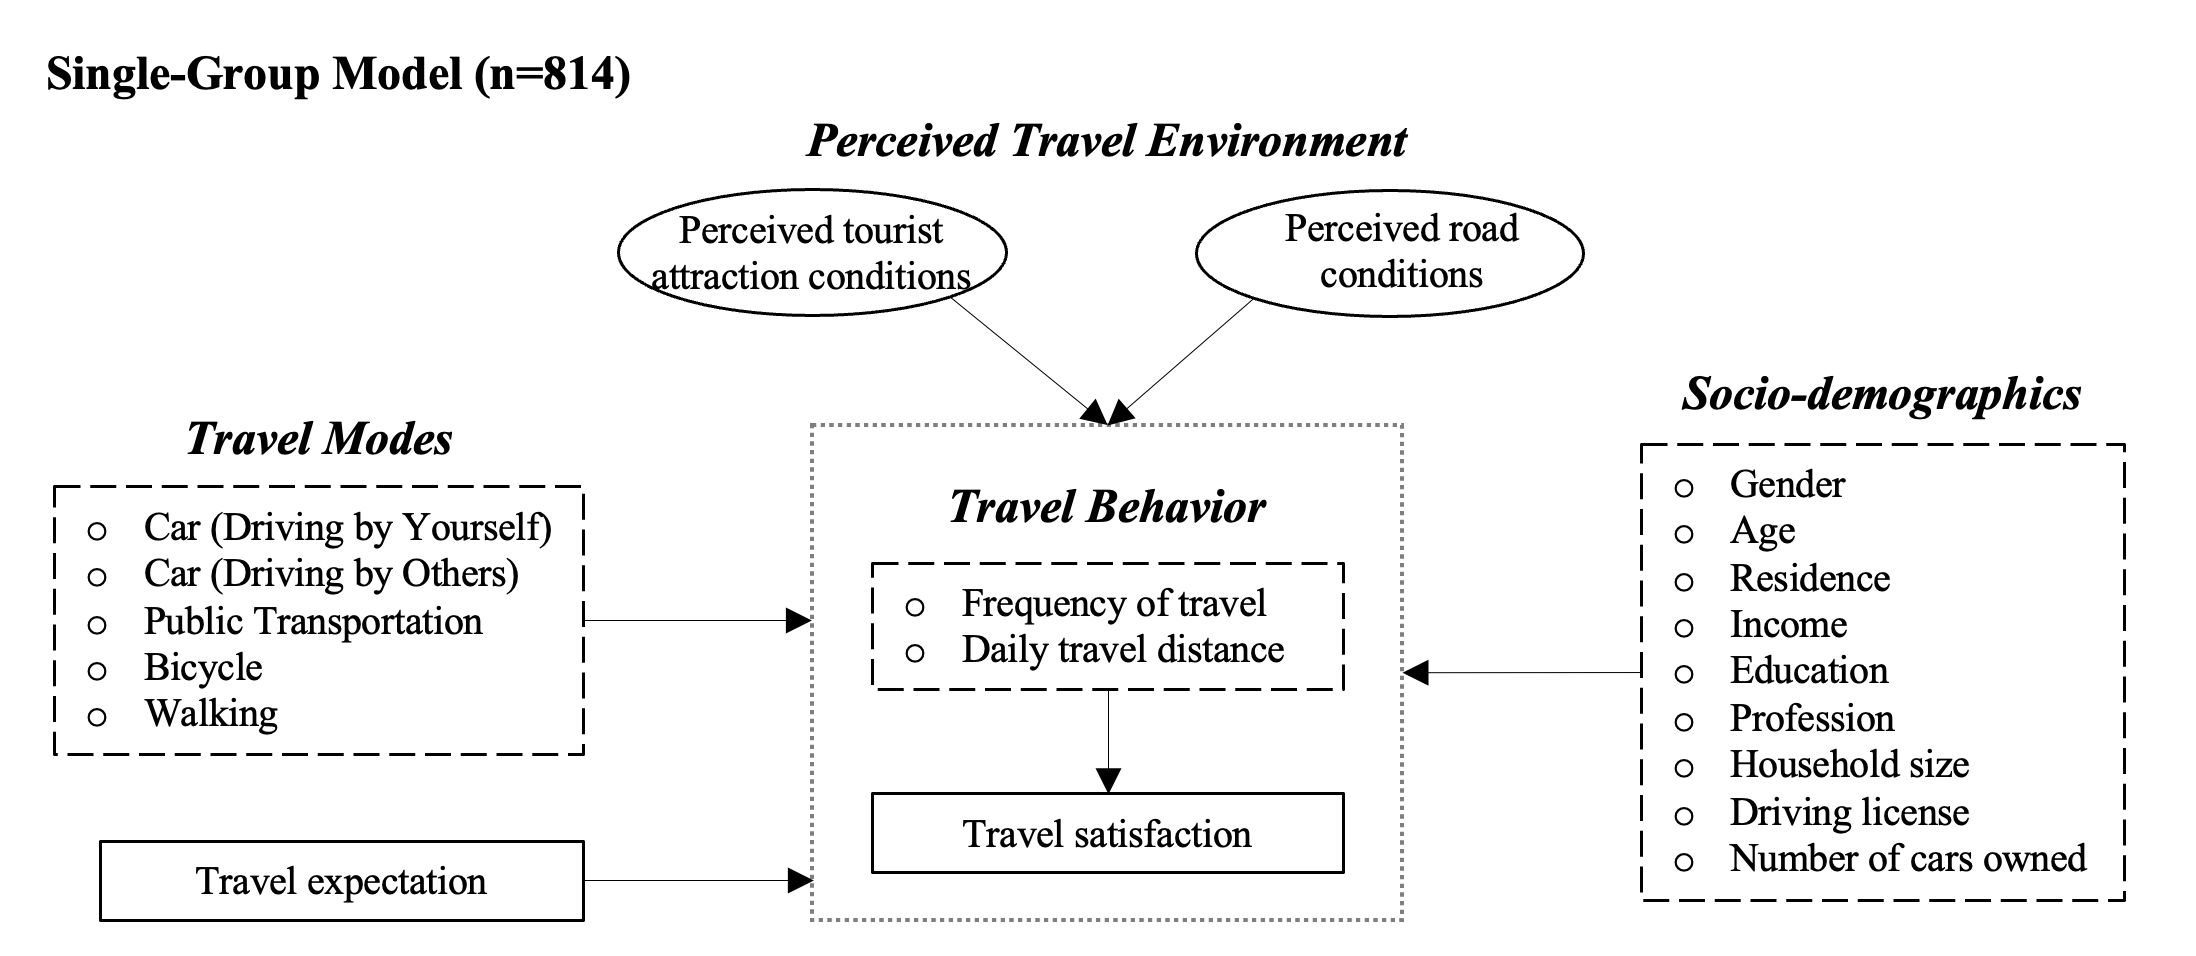
\includegraphics[width=0.8\linewidth]{figure/conceptual_framework} 

}

\caption{\label{fig:conceptual_framework} Conceptual Framework}\label{fig:fig2-conceptual-frmework}
\end{figure}

\section{Modeling}\label{modeling}

Below, confirmatory Factor Analysis (CFA) model and Structural Equation Modeling (SEM) model are respectively defined and measured.

\begin{Shaded}
\begin{Highlighting}[]
\CommentTok{\# Define the CFA model}
\NormalTok{cfa\_model }\OtherTok{\textless{}{-}} \StringTok{"}
\StringTok{\# Measurement model}
\StringTok{tourist\_envi =\textasciitilde{} ta\_envi1 + ta\_envi2 + ta\_envi3 + ta\_envi4 + ta\_envi5 }
\StringTok{  + ta\_envi6}
\StringTok{road\_envi =\textasciitilde{} r\_envi1 + r\_envi2 + r\_envi3 + r\_envi4 + r\_envi5}
\StringTok{"}

\CommentTok{\# Fit the model}
\NormalTok{fit\_cfa }\OtherTok{\textless{}{-}} \FunctionTok{cfa}\NormalTok{(cfa\_model, }\AttributeTok{data =}\NormalTok{ TBQT, }\AttributeTok{missing =} \StringTok{"ml"}\NormalTok{)}

\CommentTok{\# Model summary}
\NormalTok{cfa\_summary }\OtherTok{\textless{}{-}} \FunctionTok{summary}\NormalTok{(fit\_cfa, }\AttributeTok{fit.measures =} \ConstantTok{TRUE}\NormalTok{, }\AttributeTok{standardized =} \ConstantTok{TRUE}\NormalTok{)}
\end{Highlighting}
\end{Shaded}

\begin{Shaded}
\begin{Highlighting}[]
\CommentTok{\# Define the SEM model}
\NormalTok{model }\OtherTok{\textless{}{-}} \StringTok{"}
\StringTok{\# Measurement model}
\StringTok{tourist\_envi =\textasciitilde{} ta\_envi1 + ta\_envi2 + ta\_envi3 + ta\_envi4 + ta\_envi5 }
\StringTok{  + ta\_envi6}
\StringTok{road\_envi =\textasciitilde{} r\_envi1 + r\_envi2 + r\_envi3 + r\_envi4 + r\_envi5}

\StringTok{\# Structural model}
\StringTok{frequency\_travel \textasciitilde{} tourist\_envi + road\_envi}
\StringTok{  + self\_drive + other\_drive + pub\_trans + bicycle + walking}
\StringTok{  + exp\_lvl}
\StringTok{  + gender + age + residence + income + edu\_lvl }
\StringTok{  + profession + household\_size + dri\_lic + num\_cars}
\StringTok{daily\_d \textasciitilde{} tourist\_envi + road\_envi}
\StringTok{  + self\_drive + other\_drive + pub\_trans + bicycle + walking}
\StringTok{  + exp\_lvl}
\StringTok{  + gender + age + residence + income + edu\_lvl }
\StringTok{  + profession + household\_size + dri\_lic + num\_cars}
\StringTok{sati\_lvl \textasciitilde{} tourist\_envi + road\_envi}
\StringTok{  + self\_drive + other\_drive + pub\_trans + bicycle + walking}
\StringTok{  + exp\_lvl}
\StringTok{  + frequency\_travel + daily\_d}
\StringTok{  + gender + age + residence + income + edu\_lvl }
\StringTok{  + profession + household\_size + dri\_lic + num\_cars}

\StringTok{\# Correlations}
\StringTok{r\_envi1 \textasciitilde{}\textasciitilde{} r\_envi2}
\StringTok{exp\_lvl \textasciitilde{}\textasciitilde{} tourist\_envi}
\StringTok{ta\_envi1 \textasciitilde{}\textasciitilde{} ta\_envi2}
\StringTok{ta\_envi5 \textasciitilde{}\textasciitilde{} ta\_envi6}
\StringTok{"}

\CommentTok{\# Fit the model}
\NormalTok{fit\_sem }\OtherTok{\textless{}{-}} \FunctionTok{sem}\NormalTok{(model, }\AttributeTok{data =}\NormalTok{ TBQT, }\AttributeTok{estimator =} \StringTok{"MLR"}\NormalTok{, }\AttributeTok{std.lv =} \ConstantTok{TRUE}\NormalTok{, }\AttributeTok{missing =} \StringTok{"ml"}\NormalTok{)}

\CommentTok{\# Model summary}
\NormalTok{sem\_summary }\OtherTok{\textless{}{-}} \FunctionTok{summary}\NormalTok{(fit\_sem, }\AttributeTok{fit.measures =} \ConstantTok{TRUE}\NormalTok{, }\AttributeTok{standardized =} \ConstantTok{TRUE}\NormalTok{, }\AttributeTok{modindices =} \ConstantTok{TRUE}\NormalTok{)}

\NormalTok{mi }\OtherTok{\textless{}{-}} \FunctionTok{modindices}\NormalTok{(fit\_sem, }\AttributeTok{sort =} \ConstantTok{TRUE}\NormalTok{, }\AttributeTok{maximum.number =} \DecValTok{20}\NormalTok{)}
\end{Highlighting}
\end{Shaded}

As all of the variables in the model are categorical variables (either binary, categorical or ordinal), \texttt{lavaan} package only need to maintain the types of these categorical variables as \texttt{numeric} to deal with exogenous categorical variables. For endogenous variables, the ideal way is to set it as \texttt{ordered}, however, since the Full Information Maximum Likelihood method of dealing with missing value cannot deal with categorical variable. Therefore, I prioritized using Maximum Likelihood with Robust Standard Errors (MLR) estimator with setting \texttt{missing\ =\ "ml"} to deal with missing values.

For iterations, as the iterations control is already built into the \texttt{lavaan} package, it will automatically iterate until convergence. Regarding bootstrapping strategy, it helps to deal with data non-normality problem and to test indirect effects by estimating bias-corrected confidence intervals (CI). This method should be tested with trials, yet due to time constraints, it is not included in this model paper.

\chapter{Results}\label{rmd-basics}

\section{CFA Results}\label{cfa-results}

Confirmatory Factor Analysis (CFA) is performed at first to detect if the model can build ``perceived tourist attraction environment'' and ``perceived road environment'' as two latent variables. The method models how a set of observed variables relates to one or more latent variables.

According to CFA results (\ref{tab:cfa-model-fit}), model fit is relatively acceptable. The significant Chi-Square test (p \textless{} 0.001) is not unexpected given the large sample size (n = 814). The SRMR (0.040) indicates a good fit, and the CFI (0.926) and TLI (0.905) are close to the acceptable threshold of 0.90, suggesting a moderately acceptable fit overall. However, the RMSEA (0.094) exceeds the typical cutoff of 0.08, meaning that there could be refinements about constructing the two latent variables.

\begin{table}

\caption{\label{tab:cfa-model-fit}\label{tab:cfa-model-fit} CFA model fit results: Travel Environment variables}
\centering
\begin{tabular}[t]{lll}
\toprule
Index & Value & Standard\\
\midrule
Chi-Square & 352.57 & -\\
Degrees of Freedom & 43 & -\\
P-value (Chi-square) & <0.001 & > 0.05\\
CFI & 0.926 & >= 0.90 (acceptable)\\
TLI & 0.905 & >= 0.90 (acceptable)\\
\addlinespace
RMSEA & 0.094 & < 0.08 (acceptable)\\
P-value RMSEA <= 0.05 & 0 & > 0.05\\
SRMR & 0.04 & < 0.08 (acceptable)\\
\bottomrule
\end{tabular}
\end{table}

Regarding loading estimates, Table \ref{tab:cfa_loadings} shows that the observed variables load strongly onto their respective latent variables, indicating good measurement. For the ``perceived tourist attraction environment'' latent variable, standardized loadings range from 0.601 to 0.723, with \texttt{ta\_envi2} (``I think there is a large variety of scenic views along the route''), \texttt{ta\_envi3} (``I think the attractions I visited are well-known''), and \texttt{ta\_envi4} (``I think the scenery along the route is unique'') showing the strongest relationships. Similarly, for the perceived road environment latent variable, loadings are consistently high as well, ranging from 0.686 to 0.888, with \texttt{r\_envi4} (``The level and capability of traffic management along the route affected this trip'') and \texttt{r\_envi3} (``The availability of roadside service facilities (e.g., shops, parking lots, gas stations) affected this trip'') being the most strongly associated indicators.

\newpage
\blandscape

\begin{table}

\caption{\label{tab:cfa-loadings}\label{tab:cfa_loadings} Standardized coefficients of the measurement models}
\centering
\begin{tabular}[t]{llrrr}
\toprule
Latent Variable & Observed Variable & Coeficient & S.E. & t-statistic\\
\midrule
Perceived Tourist Attraction Environment & ta\_envi1 & 0.674 & 0.000 & NA\\
 & ta\_envi2 & 0.715 & 0.077 & 17.335\\
 & ta\_envi3 & 0.691 & 0.079 & 16.261\\
 & ta\_envi4 & 0.723 & 0.075 & 17.249\\
 & ta\_envi5 & 0.637 & 0.087 & 15.041\\
\addlinespace
 & ta\_envi6 & 0.601 & 0.086 & 14.449\\
Perceived Road Environment & r\_envi1 & 0.686 & 0.000 & NA\\
 & r\_envi2 & 0.775 & 0.056 & 20.648\\
 & r\_envi3 & 0.823 & 0.059 & 20.499\\
 & r\_envi4 & 0.888 & 0.061 & 21.456\\
\addlinespace
 & r\_envi5 & 0.814 & 0.065 & 20.511\\
\bottomrule
\multicolumn{5}{l}{\rule{0pt}{1em}\textit{Note: }}\\
\multicolumn{5}{l}{\rule{0pt}{1em}S.E. represents for standard error.}\\
\multicolumn{5}{l}{\rule{0pt}{1em}All loadings of observable variables except the first one of each latent variable are statistically significant (p < 0.001).}\\
\end{tabular}
\end{table}

\elandscape
\newpage

The covariance between the two latent variables (standardized = 0.136) is significant (p = 0.001), suggesting a moderate correlation. This indicates that individuals who perceive tourist attractions favorably also tend to rate road environments positively. And later in SEM model the two latent variables that have residual correlations are linked with \texttt{\textasciitilde{}\textasciitilde{}} symbol.

\section{SEM Results}\label{sem-results}

The Structural Equation Modeling (SEM) model demonstrates a good overall fit in Table \ref{tab:sem-model-fit}. The Chi-Square/df ratio of 2.003 is within the acceptable range (\textless{} 5), indicating a reasonable relative model fit. While indices as CFI (0.955) and TLI (0.942), exceed the threshold of 0.90, suggesting a strong fit. The RMSEA of 0.036, with a 90\% confidence interval of {[}0.031, 0.041{]}, is well below the acceptable limit of 0.08. Additionally, the SRMR of 0.042 meets the recommended standard (\textless{} 0.08). These results collectively indicate that the hypothesized model aligns well with the observed data.

\begin{table}

\caption{\label{tab:sem-model-fit}\label{tab:sem-model-fit} SEM model fit results}
\centering
\begin{tabular}[t]{lll}
\toprule
Index & Value & Standard\\
\midrule
Chi-Square & 492.814 & -\\
Degrees of Freedom & 246 & -\\
Chi-Square/df & 2.003 & < 5.0 (acceptable)\\
P-value (Chi-square) & < 0.001 & > 0.05\\
CFI & 0.955 & >= 0.90 (acceptable)\\
\addlinespace
TLI & 0.942 & >= 0.90 (acceptable)\\
RMSEA & 0.036 & < 0.08 (acceptable)\\
90\% CI RMSEA (Lower) & 0.031 & -\\
90\% CI RMSEA (Upper) & 0.041 & -\\
P-value RMSEA <= 0.05 & 1 & > 0.05\\
\addlinespace
SRMR & 0.042 & < 0.08 (acceptable)\\
\bottomrule
\multicolumn{3}{l}{\rule{0pt}{1em}\textit{Note: }}\\
\multicolumn{3}{l}{\rule{0pt}{1em}CFI = comparative fit index;}\\
\multicolumn{3}{l}{\rule{0pt}{1em}TLI = Tucker Lewis index;}\\
\multicolumn{3}{l}{\rule{0pt}{1em}RMSEA = root mean square error of approximation;}\\
\multicolumn{3}{l}{\rule{0pt}{1em}SRMR = standardized root mean square residual.}\\
\end{tabular}
\end{table}

According to the overall single-group SEM results that considered all observations (Table \ref{tab:sem-loadings}), the overall effects between different pathways are mixed.

\newpage
\blandscape

\begin{table}

\caption{\label{tab:sem-loadings}\label{tab:sem-loadings} SEM model results}
\centering
\begin{tabular}[t]{lllll}
\toprule
Sections & X. & Trip.frequency & Daily.traveling.distance & Travel.satisfaction\\
\midrule
Travel Environment & Tourist environment & -0.008 & 0.114*** & 0.448***\\
 & Road environment & -0.003 & -0.069** & -0.003\\
Travel Modes & Car (Driving by Yourself) & -0.028 & 0.247*** & -0.033\\
 & Car (Driving by Others) & -0.022 & 0.127** & -0.074\\
 & Public transportation & -0.028** & -0.138*** & -0.046\\
\addlinespace
 & Bicycle & 0.001 & 0.019 & -0.004\\
 & Walking & 0.024 & -0.095*** & 0.053*\\
Travel Expectation & Travel expectation & -0.035 & 0.025 & 0.166***\\
Travel Behavior & Frequency of travel & NA & NA & 0.063\\
 & Daily travel distance & NA & NA & -0.013\\
\addlinespace
Socio-demographics & Gender & -0.012 & -0.063** & 0.06*\\
 & Age & -0.037 & -0.016 & -0.08**\\
 & Residence & 0.75*** & -0.202*** & -0.166***\\
 & Income & 0.015 & 0.082* & 0.039\\
 & Education level & -0.017 & 0.051 & -0.006\\
\addlinespace
 & Profession & 0.046* & 0.034 & 0.039\\
 & Household size & 0.027 & 0.016 & -0.012\\
 & Owing driving licence & 0.004 & 0.097** & 0.015\\
 & Number of cars & -0.024 & 0.028 & 0\\
\bottomrule
\multicolumn{5}{l}{\rule{0pt}{1em}\textit{Note: }}\\
\multicolumn{5}{l}{\rule{0pt}{1em}All results are standardized.}\\
\multicolumn{5}{l}{\rule{0pt}{1em}***: Significant at the 0.01 level (p-value < 0.01)}\\
\multicolumn{5}{l}{\rule{0pt}{1em}**: Significant at the 0.05 level (p-value < 0.05)}\\
\multicolumn{5}{l}{\rule{0pt}{1em}*: Significant at the 0.1 level (p-value < 0.1)}\\
\end{tabular}
\end{table}

\elandscape
\newpage

\subsection{The effects of perceived travel environment on travel satisfaction}\label{the-effects-of-perceived-travel-environment-on-travel-satisfaction}

The results showed that perceived tourist attraction environment had a direct effect on travel satisfaction (0.448) while perceived road environment (-0.003) showed no such significant correlations. The better perceptions people had over the quality and other characteristics of tourist attractions, the higher satisfactory levels they tended to possess during the trip. Though, in terms of perceived road environment, the associations were weak.

Considering the mediating effects, perceived travel environment affect travel satisfaction through travel behavior. It shows that, better tourist site conditions (0.114) led to farther daily travel distance while worse road conditions (-0.069) caused people to travel less. Meanwhile, there existed no associations was obtained between travel environment and trip frequency.

\subsection{The effects of travel modes on travel satisfaction}\label{the-effects-of-travel-modes-on-travel-satisfaction}

Different levels of tourists' travel satisfaction were observed in five different travel modes, despite the relationships being mostly not significant. Walking (0.053) is the only travel mode that contributed to leveling up satisfaction, while the other four (i.e., car driving by yourself, car driving by others, public transportation, and bicycle) all resulted in not significant lower satisfaction, with car driving by others (-0.074) lowering the most.

Regarding the influence travel modes exerted on travel behavior, daily travel distance was generally more associated with travel modes compared to trip frequency. Car, either driven by yourself (0.247), car driven by others (0.127), both significantly caused tourists to travel longer distance, while the former has bigger influence than the latter. Meanwhile, public transit (-0.138) and walking (-0.095) both significantly discouraged tourists from traveling farther. For the effects of travel modes on travel frequency, public transportation (-0.028) is associated with lowering people's intentions of traveling. While for other travel modes, driving by car will lower travel frequency while walking will boost it, though none of them are significant, meaning that there exist no mediating effects towards travel satisfaction either.

\subsection{The effects of travel behavior on travel satisfaction}\label{the-effects-of-travel-behavior-on-travel-satisfaction}

In terms of travel behavior, our study only considered two variables - tourists' trip frequency to Qinghai-Tibet Plateau and their daily travel distance during the trip. The results showed that higher frequency of travelling to Qinghai-Tibet Plateau had a direct positive effect (0.063) on tourist travel satisfaction, despite the correlation being not significant. This could indicate that as tourists travel to Qinghai-Tibet Plateau more times their satisfactory levels would steadily improve. However, the associations between daily travel distance and travel satisfaction were not significant. This might result in the gradient setting of daily traveling distance in the questionnaire (distance categorized as \textless10 km, 10-50 km, 50-100 km, 100-200 km, \textgreater200 km). However, based on the simple statistical analysis of the average tourists' satisfactory levels under different distance gradients, it was found that distance-satisfaction relationship might follow a U-shaped pattern as shown in Figure \ref{fig:sati-by-distance}.

\begin{figure}

{\centering 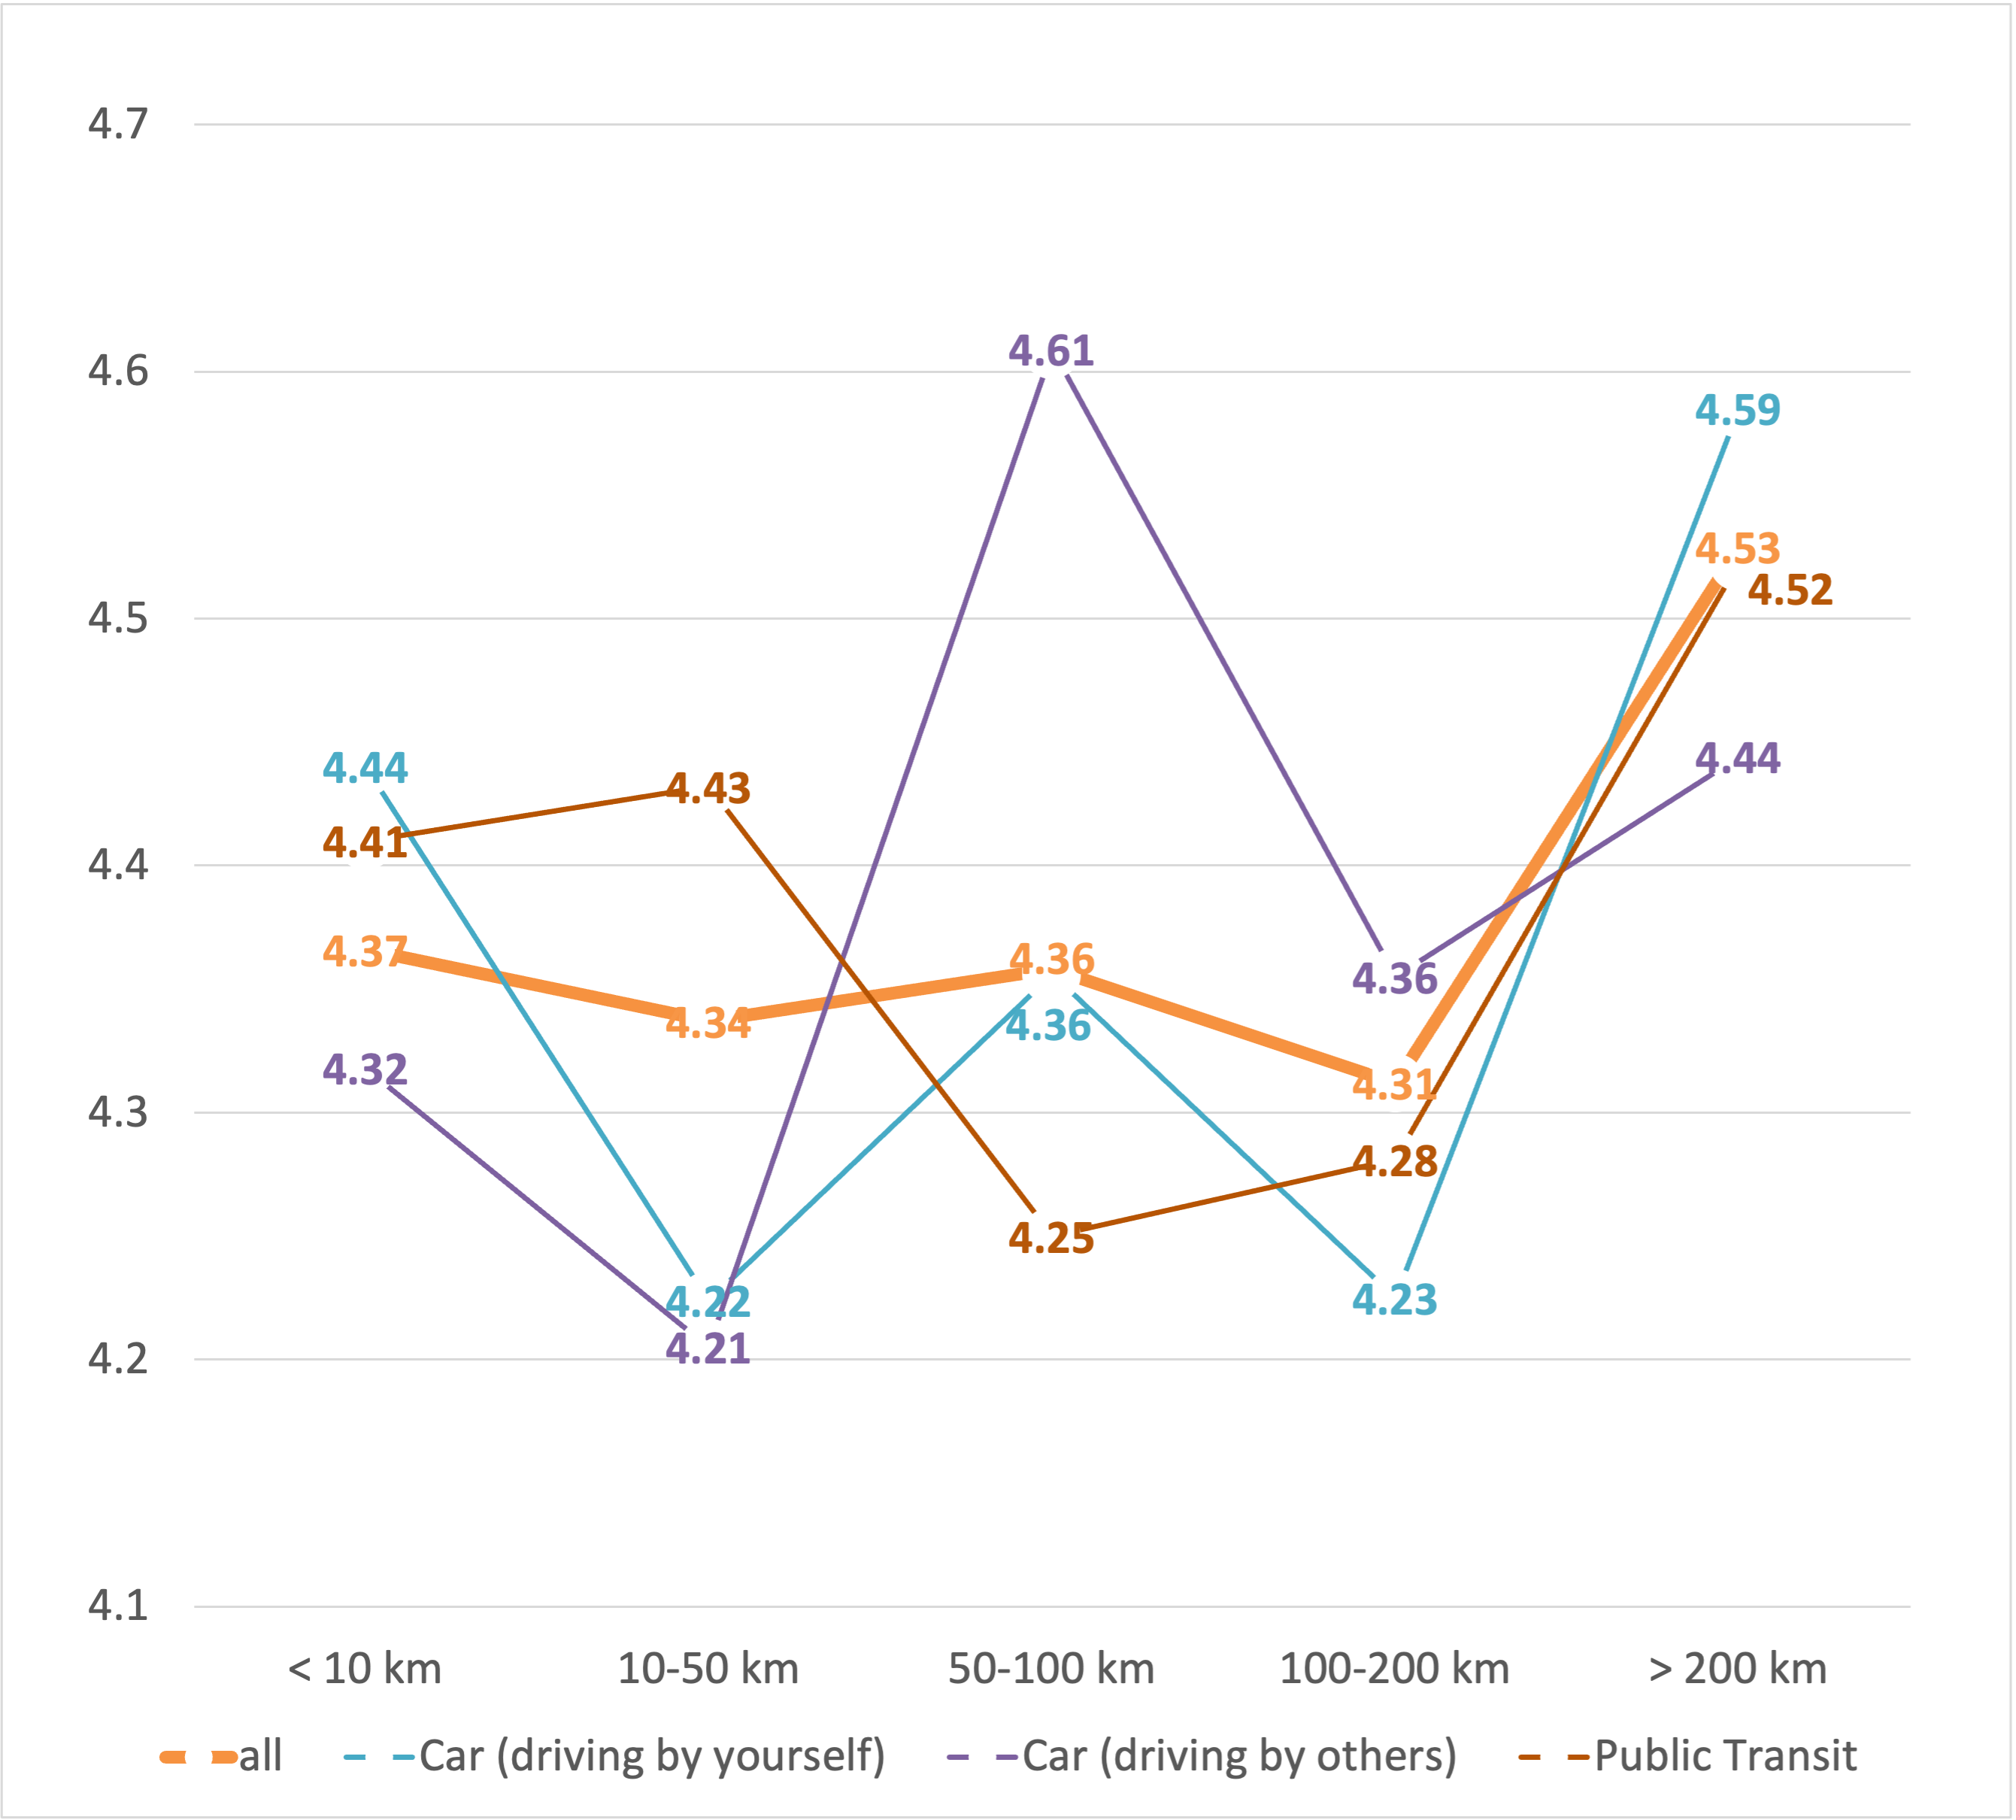
\includegraphics[width=0.8\linewidth]{figure/sati-by-distance} 

}

\caption{\label{fig:sati-by-distance} Travle satisfaction by gradient travel distance levels}\label{fig:fig3-sati-by-distance}
\end{figure}

For the single-group scenario, within the 200 kilometers range, tourists' satisfactory levels fluctuated and slightly decreased (from 4.366 for \textless10 km to 4.312 for 100-200 km) as they traveled longer distance. However, the pattern displayed a drastic surge of satisfactory levels when travel distance exceeded 200 kilometers. The possible cause for the decrease could be attributed to increasing fatigue of sitting or driving during daily travelling. While for the surge, it is speculated that the beauty and uniqueness of natural landscapes of Qinghai-Tibet Plateau had positive effects on travelers' eyes and moods, which would first offset the tiredness brought by means of transport and then improve tourists' satisfactory levels. This pattern was also observed in studies of (Ettema et al., 2011), who theorized that the positive relationships between distance and satisfaction could be ascribed to the inner vales contained activities in travel (e.g., admiring scenery, listening to music, having fun, etc.). Furthermore, considering the huge area of Qinghai-Tibet Plateau and the percentage of people traveling in cars (62.3\%), the 200 kilometers could be an important distance demarcating point, where visual contentment gained along the road would prevail over physical fatigue thus leading satisfactory levels to rise.

\subsection{Effects of travel expectation and socio-demographics on travel satisfaction}\label{effects-of-travel-expectation-and-socio-demographics-on-travel-satisfaction}

The results showed that travel expectation had a significantly positive effect (0.166) on travel satisfaction only directly. The highly anticipated travel with big expectations before traveling tended to result in higher levels of satisfaction. However, as travel expectation does not has dierect influence over travel bahvior, there seems to be no mediating effects on travel satisfaction.

In terms of socio-demographics, both direct and indirect effects demonstrated high heterogeneity in different paths. The binary exogenous variable residence, which reflected different sources of tourists (0 for non-local, 1 for local), proved to be an important factor that influenced both travel satisfaction and travel behavior. Local people generally had lower satisfactory levels over the course of their whole travel experience compared to non-locals (-0.166). The cause for this might stem from people's different travel intentions. Taking planned travel time for example, 49.3\% non-local people planned to travel longer than a week, while the majority local people (85.0\%) only planned one-week travel or even shorter. Further, there could exist hidden factors (i.e., varied subjective well-being levels) that account for the results, regarding income, profession, education, etc. Simultaneously, local people significantly travel more frequently and within shorter distance, which can be regarded as supplementary evidence of different travel intentions.

For other socio-demographic characteristics, women (0.06) and younger people (-0.08) had higher levels of travel satisfaction, and people who have higher income, better education and more flexible professions also tended to be more satisfactory, though the latter paths were not significant. Considering the effects on travel behavior, those who have inflexible professions (0.046) tend to travel more frequently, while men (-0.063) and people with higher income (0.083), as well as owning a driving license (0.097) would travel longer distance.

\chapter*{Conclusion}\label{conclusion}
\addcontentsline{toc}{chapter}{Conclusion}

The study probes into how factors as travel behavior and perceived travel environment can influence tourists' travel satisfaction on Qinghai-Tibet Pleateau. The single-group SEM analysis conducted in this model peper revealed mixed effects across different pathways. Perceived tourist attraction environment significantly influenced travel satisfaction, while perceived road environment had no notable direct effect. Mediating effects showed that better tourist site conditions led to longer daily travel distances, whereas worse road conditions reduced travel distance. Travel modes exhibited minimal direct effects on satisfaction, with walking positively contributing and car driving by others showing the largest negative impact. Regarding travel behavior, frequency of travel to the Qinghai-Tibet Plateau had a minor positive effect on satisfaction, although insignificant, and daily travel distance showed no direct association.

The innovative highlights of the study would be using SEM modeling to comprehensively incorporate all relevant factors that could impact travel satisfaction. While it focused on the perspectives of tourism traveling instead of work commuting, a travel activity that has been well researched and concentrated on. Meanwhile, the study supplements the vacancy of similar travel behavior related studies conducted on a plateau area, as most focuses on cities of low altitude.

There are also some aspects this article can be further improved: 1) if conducting follow-up survey or new survey projects targeted at travel satisfaction, the more standardized and official survey scale, such as Satisfaction with Travel Scale (STS) by Ettema et al. (2011), could be used; 2) objective and measurable traveling time, distance, and road infrastructure geo-spatial data could be calculated and added into this study, however, it is true that such data might not be easy to obtain due to harsh natural environments and governments' privacy concerns; 3) Could further dig into the dynamic intersecting influences between variables by performing multiple-group models using variables such as residence, profession, or travel modes.

\backmatter

\chapter*{References}\label{references}
\addcontentsline{toc}{chapter}{References}

\markboth{References}{References}

\noindent

\setlength{\parindent}{-0.20in}
\setlength{\leftskip}{0.20in}
\setlength{\parskip}{8pt}

\phantomsection\label{refs}
\begin{CSLReferences}{1}{0}
\bibitem[\citeproctext]{ref-Bollen1989}
Bollen, K. A. (1989). Structural equation models with observed variables. In \emph{Structural equations with latent variables} (pp. 80--150). John Wiley \& Sons, Ltd. http://doi.org/\href{https://doi.org/10.1002/9781118619179.ch4}{10.1002/9781118619179.ch4}

\bibitem[\citeproctext]{ref-Carneiro2019}
Carneiro, M. J., \& Eusébio, C. (2019). Factors influencing the impact of tourism on happiness. \emph{Anatolia}, \emph{30}(4), 475--496. http://doi.org/\href{https://doi.org/10.1080/13032917.2019.1632909}{10.1080/13032917.2019.1632909}

\bibitem[\citeproctext]{ref-Chen2019}
Chen, S., Fan, Y., Cao, Y., \& Khattak, A. (2019). Assessing the relative importance of factors influencing travel happiness. \emph{Travel Behaviour and Society}, \emph{16}, 185--191. http://doi.org/\href{https://doi.org/10.1016/j.tbs.2019.01.002}{10.1016/j.tbs.2019.01.002}

\bibitem[\citeproctext]{ref-DeVos2019}
De Vos, J. (2019). Analysing the effect of trip satisfaction on satisfaction with the leisure activity at the destination of the trip, in relationship with life satisfaction. \emph{Transportation}, \emph{46}, 623--645. http://doi.org/\href{https://doi.org/10.1007/s11116-017-9812-0}{10.1007/s11116-017-9812-0}

\bibitem[\citeproctext]{ref-Diener2000}
Diener, E. (2000). Subjective well-being: The science of happiness and a proposal for a national index. \emph{American Psychologist}, \emph{55}(1), 34--43.

\bibitem[\citeproctext]{ref-Ettema2011}
Ettema, D., Gärling, T., Eriksson, L., Friman, M., Olsson, L. E., \& Fujii, S. (2011). Satisfaction with travel and subjective well-being: Development and test of a measurement tool. \emph{Transportation Research Part F: Traffic Psychology and Behaviour}, \emph{14}(3), 167--175. http://doi.org/\href{https://doi.org/10.1016/j.trf.2010.11.002}{10.1016/j.trf.2010.11.002}

\bibitem[\citeproctext]{ref-Gao2021}
Gao, X., \& Sun, D. (2021). Transport accessibility and social demand: A case study of the tibetan plateau. \emph{PLOS ONE}, \emph{16}(9), e0257028. http://doi.org/\href{https://doi.org/10.1371/journal.pone.0257028}{10.1371/journal.pone.0257028}

\bibitem[\citeproctext]{ref-Hayes2009}
Hayes, A. F. (2009). Beyond baron and kenny: Statistical mediation analysis in the new millennium. \emph{Communication Monographs}, \emph{76}(4), 408--420. http://doi.org/\href{https://doi.org/10.1080/03637750903310360}{10.1080/03637750903310360}

\bibitem[\citeproctext]{ref-McCabe2013}
McCabe, S., \& Johnson, S. (2013). The happiness factor in tourism: Subjective well-being and social tourism. \emph{Annals of Tourism Research}, \emph{41}, 42--65. http://doi.org/\href{https://doi.org/10.1016/j.annals.2012.12.001}{10.1016/j.annals.2012.12.001}

\end{CSLReferences}

\end{document}
